\section{Bewerkingen}

\subsection{Volgorde van bewerkingen}
Om een opgave juist te kunnen oplossen, is het noodzakelijk om de volgorde van de bewerkingen te respecteren:

\begin{enumerate}
	\item \textbf{H}aakjes
	\item \textbf{M}achten en worteltrekken
	\item \textbf{W}issel van teken
	\item \textbf{V}ermenigvuldigen en \textbf{d}elen (dezelfde prioriteit)
	\item \textbf{O}ptellen en \textbf{a}ftrekken (dezelfde prioriteit)
\end{enumerate}

Let op! Haakjes staan voor deelopgaven die je eerst moet maken, hierop moet je inzoomen.

\subsubsection{Opmerkingen}
\begin{itemize}
	\item Bewerkingen met dezelfde prioriteit worden van links naar rechts uitgevoerd.
	\item Een ezelsbruggetje om dit te onthouden: \textbf{H}oe \textbf{M}oeten \textbf{W}ij \textbf{V}an \textbf{D}e \textbf{O}nvoldoendes \textbf{A}fkomen?
	\item Machtsverheffen gaat voor op tekenwisseling: als je $-5^2$ moet uitrekenen, doe je eerst $5^2=25$ en daarna pas je op het resultaat de tekenwisseling toe zodat het antwoord $-25$ wordt.
	\item Bedoel je echter het kwadraat van $-5$ dan noteer je $(-5)^2=(-5).(-5)=25$
\end{itemize}

\subsection{Volgorde van bewerkingen - voorbeeld 1}
Zie filmpje MOOC.

\subsection{Volgorde van bewerkingen - voorbeeld 2}
Zie filmpje MOOC.

\subsection{Rekenen met machten of exponenten}
\subsubsection{Wat is een macht?}
De vermenigvuldiging is ingevoerd om de schrijfwijze bij een optelling te vereenvoudigen. Immers:
\begin{equation*}
\underbrace{4+4+4+4+4+4}_{\text{6 maal}}
\end{equation*}
was vervelend om te schrijven. Omdat de 4 zesmaal voorkomt, werd dit $6 \cdot 4$.

Later werd er dan ook gedefinieerd wat het betekende om kommagetallen met mekaar te vermenigvuldigen.

Machten zijn ingevoerd om volgende schrijfwijzes eenvoudiger te maken:
\begin{equation*}
\underbrace{4 \cdot 4\cdot4\cdot4\cdot4\cdot4}_{\text{6 maal}}
\end{equation*}
In plaats van een som van dezelfde getallen, hebben we nu een product van dezelfde getallen.

Verkort geschreven wordt dit: $4^6$

Een macht bestaat uit twee delen: een exponent, hier $6$ en een grondtal, hier $4$.

Het grondtal mag (mits enkele uitzonderingen) elk re\"eel getal zijn. De exponent mag eigenlijk (ook weer met enkele uitzonderingen) elk re\"eel getal zijn. Om de volgorde van bewerkingen uit te leggen, gebruiken we in dit hoofdstuk enkel natuurlijke (gehele) exponenten.

\begin{voorbeeld}
	\begin{equation*}
	12+3^2 \cdot 4 : 2 - 8 : 4 + 3 - 5^2
	\end{equation*}
	Hoe pakken we dit nu aan? We zien dat er enkele machten in staan, dus die rekenen we eerst uit. Vervolgens rekenen we alle vermenigvuldigingen en delingen uit, van links naar rechts. Dan doen we alle optellingen en aftrekkingen, van links naar rechts.
	\begin{equation*}
	\begin{array}{lllr}
	12+\underbrace{3^2}_{9} \cdot 4 : 2 - 8 : 4 + 3 - \underbrace{5^2}_{25} &=& 12+ \underbrace{9 \cdot 4}_{36} : 2 - \underbrace{8 : 4}_{2} + 3 - 25 & \text{vermenigvuldigen en delen} \\
	&=& 12+ \underbrace{36 : 2}_{18} - 2 + 3 - 25 & \text{vermenigvuldigen en delen} \\
	&=& \underbrace{12+18} _{30} - 2 + 3 - 25 & \text{optellen en aftrekken} \\
	&=& \underbrace{30 - 2}_{28} + 3 - 25 & \text{optellen en aftrekken} \\
	&=& \underbrace{28+3}_{31} - 25 & \text{optellen en aftrekken} \\
	&=& 31 - 25 & \text{optellen en aftrekken} \\
	&=& 6 &  \\
	\end{array}
	\end{equation*}
\end{voorbeeld}


\subsection{Werken met haakjes}
\subsubsection{Wat als er haakjes staan?}

Haakjes zijn nuttig om aan te duiden dat de bewerking ertussen eerst moet gebeuren. Haakjes zullen dus voorrang hebben op alles.

\fbox{\begin{minipage}{\linewidth}
	Onthoud \\
	
	Los eerst alles tussen de haakjes op!	
	\end{minipage}}

Haken symboliseren in feite een deelopgave. Ze verplichten je eerst die deelopgave op te lossen, vooraleer je de grote oplossing mag starten.


\begin{voorbeeld}
\begin{equation*}
6 \cdot (4+5) = 6 \cdot 9 = 54
\end{equation*}	
	
In deze opgave is $(4 + 5)$ de deelopgave, dus die los je eerst op en je vult het resultaat in. 
Dan ga je gewoon verder met de rest van de opgave.

Even vergelijken wat er gebeurt als er geen haken staan, dus dan moet je eerst de vermenigvuldiging uitwerken:

\begin{equation*}
6 \cdot 4+5 = 24+5=29
\end{equation*}	

Iets totaal anders!

Let op: $6 \cdot (4+5) \ne 6\cdot 4+5$

\end{voorbeeld}

\begin{voorbeeld}

\begin{equation*}
\begin{array}{ccrl}
20 : 4 \cdot 5 &=& 20:20 =1 & \text{is fout,} \\
20 : 4 \cdot 5 &=& 5 \cdot 5 =25 & \text{is juist.}
\end{array}
\end{equation*}
	
Dit soort fouten kan je voorkomen door (zelf) haakjes te gebruiken:

\begin{equation*}
(20 : 4) \cdot 5 = 5 \cdot 5 = 25
\end{equation*}

Een andere manier om dit soort problemen te omzeilen is door “delen door 4” te vervangen door “vermenigvuldigen met een vierde” en vervolgens van links naar rechts te rekenen:

\begin{equation*}
20 : 4 \cdot 5 = 20 \cdot \frac{1}{4} \cdot 5 = 25
\end{equation*}

Dit geldt ook voor de optelling en de aftrekking:

\begin{equation*}
\begin{array}{ccrl}
5-3+1 &=& 5-4 =1 & \text{is fout,} \\
5-3+1 &=& 2+1=3 & \text{is juist.}
\end{array}
\end{equation*}

Dit soort fouten kan je voorkomen door (zelf) haakjes te gebruiken:

\begin{equation*}
(5-3)+1 = 2+1=3 
\end{equation*}

Een andere manier is om dit soort problemen te omzeilen is door “aftrekken van plus 3” te vervangen door “optellen met min drie” en vervolgens van links naar rechts te rekenen:

\begin{equation*}
5-3+1 = 5+(-3)+1=3 
\end{equation*}

\end{voorbeeld}

\subsubsection{Wat als er meerdere haakjes zijn?}

\fbox{\begin{minipage}{\linewidth}
Soms kunnen er meerdere haakjes voorkomen. Er geldt dan de volgende regel: Bij meerdere haakjes, werk je eerst de binnenste uit, en dan werk je naar buiten. 

Wat is er eigenlijk aan de hand? In de deelopgave van de buitenste haakjes staan er nog meer haakjes. Dit is in feite een deelopgave in een deelopgave.

\begin{enumerate}
	\item Je start met die binnenste deelopgave.
	\item Je vult de uitkomst van die deelopgave in.
	\item Je gaat verder met de volgende deelopgave.
	\item Je vult dit weer in.
	\item Enzoverder!
\end{enumerate}
	\end{minipage}
}

\begin{voorbeeld}
\begin{equation*}
((3+6)-4^2)\cdot 2
\end{equation*}
Dit voorbeeld heeft verschillende haken (deelopgaven). Je ziet de buitenste haken. Daar is de deelopgave dus:
\begin{equation*}
((3+6)-4^2)
\end{equation*}
Binnen deze deelopgave staan nieuwe haken, dus die moet je weer eerst uitrekenen, we starten dus met het uitrekenen van de binnenste haken:
\begin{equation*}
\begin{array}{cclr}
\left( \underbrace{(3+6)}_{9}-4^2\right)\cdot 2 &=& \left( 9-\underbrace{4^2}_{16}\right)\cdot 2 & \text{machten binnen de haakjes} \\
&=& \underbrace{(9-16)}_{-7}\cdot 2 & \text{haken} \\
&=& -7 \cdot 2 & \text{min maal plus is min} \\
&=& -14
\end{array}
\end{equation*}
Let dus goed op in dit voorbeeld. Je moet haken altijd eerst uitrekenen, van binnen naar buiten.

Je moet een deelopgave (die binnen de haken staat) zelf behandelen als een opgave en dus de volgorde van bewerkingen daarbinnen toepassen.

\end{voorbeeld}
\subsection{Begrippen tegengestelde en omgekeerde van een getal}

\subsubsection{Tegengestelde}

Het \emph{tegengestelde} van een getal $n$ is het getal dat opgeteld
bij $n$, nul oplevert. Het tegengestelde van n wordt genoteerd met
$-n$. Het tegengestelde van een getal heeft dus dezelfde absolute
waarde als het gegeven getal maar met een tegengesteld teken. De som
van een getal met zijn tegengestelde is dus steeds 0: $n+(-n)=0$.

\noindent Zo is het tegengestelde van 12 gelijk aan \textminus 12
omdat 12 + (\textminus 12) = 0, en het tegengestelde van $-\sqrt{3}$
is $\sqrt{3}$ omdat $-\sqrt{3}+\sqrt{3}=0$.

\medskip{}


\noindent Het tegengestelde van nul is nul. Dit is het enige getal
waarvan het tegengestelde gelijk is aan zichzelf. 

\noindent We zeggen dat 0 het \emph{neutraal element} is met betrekking
tot optellen.

\noindent (In de abstracte algebra is het tegengestelde het inverse
element voor een bewerking die met een plusteken genoteerd wordt).

\bigskip{}

\subsubsection{Omgekeerde}

\noindent Het \emph{omgekeerde} of de \emph{reciproque} (vaker: de
reciproke) van een getal of grootheid is 1 gedeeld door dat getal
of die grootheid. Het omgekeerde van een breuk ontstaat door teller
en noemer te verwisselen. Het omgekeerde van 7 is 1/7 en het omgekeerde
van 2/3 is 3/2. Passen we dit toe op enkele grootheden: de hertz is
het omgekeerde van de seconde: 1 Hz = 1/s en de siemens is het omgekeerde
van de ohm: 1 S = 1/$\Omega$.

\noindent Het product van een getal met zijn omgekeerde levert 1 op:
${\displaystyle n.\frac{1}{n}=1}$. 

\noindent We zeggen dat 1 het \emph{neutraal element} is voor de vermenigvuldiging.
We zien ook dat nul geen omgekeerde heeft.

\noindent (In de abstracte algebra is het omgekeerde het inverse element
voor een bewerking die met een vermenigvuldigingsteken genoteerd wordt).

\medskip{}


\noindent Een interessante toepassing van het omgekeerde vinden we
bij de deling waarbij de deler een breuk is. De deling kan dan ook
uitgevoerd worden door het deeltal te vermenigvuldigingen met het
omgekeerde van de deler. 

\noindent Populair gezegd: delen door een breuk is vermenigvuldigen
met het omgekeerde.

\noindent Voorbeeld: $5:1/3=5\times3=15$ 


\subsection{Rekenen met wortels}
\subsubsection{Vierkantswortels}


Het meest gekende type van wortel is de vierkantswortel. De vierkantswortel geeft de mogelijkheid om een antwoord te vinden op de vraag: welk getal heeft als kwadraat 4? Een mogelijk antwoord is het getal 2. De vierkantswortel is de 'omgekeerde' bewerking van het kwadraat.
\begin{equation*}
\begin{array}{ccccccc}
\sqrt{9} &=& 3 & \text{want} & 3^2 &=& 9 \\
\sqrt{1} &=& 1 & \text{want} & 1^2 &=& 1 \\
\sqrt{0} &=& 0 & \text{want} & 0^2 &=& 0 
\end{array}
\end{equation*}

$\sqrt{-4}$ bestaat niet, want er is geen re\"eel getal dat als kwadraat een negatief getal heeft.

Je ziet dus duidelijk dat je geen vierkantswortel kan nemen van een strikt negatief getal. Een kwadraat is immers altijd positief.

Een vierkantswortel kan je nemen van elk positief re\"eel getal. Je kan dus ook $\sqrt{2}=1,4142\ldots$ berekenen. 
Dit is geen 'mooi' getal, maar het kwadraat is wel 2.

Eigenlijk is er nog een tweede oplossing voor het probleem "Welk getal heeft als kwadraat $4$?"
Immers, $-2$ is ook een juiste oplossing. $(-2)^2=4$, want het kwadraat van een negatief getal is positief. We spreken echter af dat het symbool van de vierkantswortel altijd een positief getal uitdrukt. Wil je dan toch een negatief getal, dan schrijf je bijvoorbeeld $-\sqrt{4}$, je zet er dus een minteken voor.


\begin{definitie}
	Een vierkantswortel van een positief re\"eel getal $x$, genoteerd als $\sqrt{x}$, is een positief re\"eel getal dat als kwadraat het getal $x$ heeft.
\end{definitie}

Vierkantswortels en kwadraten 'heffen mekaar op', of althans, dat lijkt zo: $\sqrt{3^2}=3$. Maar laat je niet vangen! $\sqrt{(-2)^2}$ is niet gelijk aan $-2$, maar gelijk aan $2$. \textbf{Vierkantswortels zijn altijd positief!} Reken voor de veiligheid altijd de haakjes uit, en gebruik niet een 'trucje' als de kwadraat en de wortel schrappen:
\begin{equation*}
\sqrt{(-2)^2}=\sqrt{4}=2
\end{equation*}

\subsubsection{Derdemachtswortels}

Als je een symbool hebt voor de omgekeerde bewerking van het kwadraat, is er ook eentje voor de derde macht. Dit noemen we de derdemachtswortel.

\begin{equation*}
\begin{array}{ccccccc}
\sqrt[3]{8} &=& 2 & \text{want} & 2^3 &=& 8 \\
\sqrt[3]{1000} &=& 10 & \text{want} & 10^3 &=& 1000 \\
\sqrt[3]{1} &=& 1 & \text{want} & 1^3 &=& 1 \\
\sqrt[3]{0} &=& 0 & \text{want} & 0^3 &=& 0 
\end{array}
\end{equation*}


Wat gebeurt er met negatieve getallen? Negatieve getallen hebben geen vierkantswortel, maar wel een derdemachtswortel. 
De derde macht van een negatief getal is zelf negatief, dus kan de omgekeerde bewerking wel!

\begin{equation*}
\begin{array}{ccccccc}
\sqrt[3]{-8} &=& -2 & \text{omdat} & (-2)^3 &=& -8 \\
\sqrt[3]{-1} &=& -1 & \text{want} & (-1)^3 &=& -1 \\
\end{array}
\end{equation*}

Net zoals bij vierkantswortels, hoeft een derdemachtswortel niet 'uit te komen', je kan het dus nemen van eender welk re\"eel getal.

\begin{definitie}
	Een derdemachtswortel van een re\"eel getal $x$, genoteerd als $\sqrt[3]{x}$, is het re\"ele getal dat als 3de macht het getal $x$ heeft.
\end{definitie}


\subsubsection{Hogere machtswortels}


Ook voor hogere machten bestaat er een omgekeerde bewerking, namelijk de hogere machtswortels. Deze noteer je op gelijkaardige manier. 
De vijfdemachtswortel van $2$ noteer je dan:
\begin{equation*}
\sqrt[5]{2}
\end{equation*}

Je moet hierbij het volgende onthouden:

\fbox{\begin{minipage}{\linewidth}
Onthoud

\begin{itemize}
	\item Een even machtswortel (waartoe ook de vierkantswortel behoort) kan je enkel nemen van positieve re\"ele getallen en is zelf positief.
	\item Een oneven machtswortel kan je nemen van elk re\"eel getal, en kan dus positief of negatief zijn.
\end{itemize}	
\end{minipage}
}

\subsubsection{Rekenregel}

De belangrijkste rekenregel met wortels is:

\fbox{\begin{minipage}{\linewidth}
		De wortel van een product, is het product van de wortels.
	\end{minipage}
}

Voorbeelden:
\begin{eqnarray*}
\sqrt{4 \cdot 9} &=& \sqrt{4}\cdot \sqrt{9} = 2 \cdot 3 = 6 \\
\sqrt[3]{2 \cdot 27} &=& \sqrt[3]{2} \cdot \sqrt[3]{27} = \sqrt[3]{2} \cdot 3 = 3 \sqrt[3]{2}
\end{eqnarray*}

Je gebruikt deze regel erg vaak om wortels te vereenvoudigen. Bij het vereenvoudigen van een wortel probeer je wat er onder de wortel staat zo klein mogelijk te maken. Een mogelijke vraag is dus: vereenvoudig $\sqrt{200}$. Van $200$ kan je niet gemakkelijk een vierkantswortel nemen. Er is echter een factor van $200$ waarvan dat wel kan, namelijk $100$, dus zonder je die factor af:
\begin{equation*}
\sqrt{200}=\sqrt{100 \cdot 2} = \sqrt{100} \cdot \sqrt{2} = 10\sqrt{2}
\end{equation*}

Omdat $\sqrt{2}$ niet meer te vereenvoudigen is, is $10\sqrt{2}$ de meest eenvoudige vorm. Het is dus een kwestie van goede factoren te vinden die het nemen van een wortel makkelijker maken. Twee andere voorbeelden:

\begin{eqnarray*}
	\sqrt{20} &=& \sqrt{4 \cdot 5} = \sqrt{4}\cdot \sqrt{5} = 2\sqrt{5}\\
	\sqrt{90} &=& \sqrt{9 \cdot 10} = \sqrt{9} \cdot \sqrt{10} = \sqrt{3} \cdot \sqrt{10}
\end{eqnarray*}


In feite breng je het 'kwadraat buiten de vierkantswortel'. Deze regel werkt dus voor alle machtswortels, dus vierkantswortels, derdemachtswortels, enzoverder. Het enige waar je mee moet opletten is dat alles bestaat. Hou er rekening mee dat je vierkantswortels (en andere even hogere machtswortels) niet kan nemen van negatieve getallen.

Getallen die dezelfde wortel hebben, noemen we \textbf{gelijksoortig}. Zo zijn  $2\sqrt{3}$ en $4\sqrt{3}$ gelijksoortig, maar zijn $4\sqrt{5}$ en $2\sqrt{2}$ dat niet. Gelijksoortige getallen kan je optellen:
Het werkt een beetje zoals eenheden. Je kan $3m^2$ en $5m^2$ optellen, maar $3m^2$ en $8cm^2$ niet zo gemakkelijk. Dan moet je ze eerst omzetten. Dat doe je dan ook bij wortels door ze te vereenvoudigen:
\begin{equation*}
\sqrt{27}+2\cdot\sqrt{3}=\sqrt{9 \cdot 3}+2\cdot \sqrt{3}=3\cdot\sqrt{3}+2\cdot\sqrt{3}=5 \cdot \sqrt{3}
\end{equation*}

\fbox{\begin{minipage}{\linewidth}
Onthoud \\

Heel belangrijk! Er bestaat geen regel voor de wortel van een som!

\begin{equation*}
\sqrt{a+b}\ne \sqrt{a} + \sqrt{b}
\end{equation*}
	\end{minipage}
}


Een voorbeeld dat dit inderdaad niet klopt:
\begin{itemize}
	\item $\sqrt{9+16}=\sqrt{25}=5$
	\item $\sqrt{9}+\sqrt{16}=3+4=7$
\end{itemize}

Maak dus geen fout zoals $\sqrt{x^2+4}=x+2$

\subsubsection{Rationale exponenten}

We hebben bij machten reeds gesproken over natuurlijke en gehele exponenten. Rationale getallen kunnen ook een exponent vormen. Dit zullen uiteindelijk een type wortel zijn. Een eerste rationale macht heb je al gezien, een voorbeeld:

\begin{equation*}
2^{1/2}=\sqrt{2}
\end{equation*}

De exponent $1/2$ symboliseert de vierkantswortel. De exponent $1/3$ zal de derdemachtswortel symboliseren.


\begin{definitie}
	
\begin{itemize}
\item De noemer van de breuk van een rationale exponent symboliseert een machtswortel.
\item De teller van de breuk van een rationale exponent symboliseert een macht.
\end{itemize}
\end{definitie}

Wat betekent dit nu? Als ik een getal, zeg $5$,verhef tot een breuk, zeg $2/3$, dan doe ik twee dingen:

\begin{enumerate}
	\item De noemer van de breuk is 3, dus ik moet een derdemachtswortel nemen.
	\item De teller van de breuk is 2, dus ik moet een tweede macht nemen (een kwadraat dus).
\end{enumerate}

Bijgevolg:

\begin{equation*}
5^{2/3} = (\sqrt[3]{5})^2 \text{ of } \sqrt[3]{5^2}
\end{equation*}

Belangrijk is dat het getal dat je tot de macht verheft, zowel een wortel als een macht over zichzelf heen krijgt, de volgorde van de twee maakt niet uit. Vaak gebruiken we de eerste schrijfwijze, omdat het dan duidelijker is als er vereenvoudigingen mogelijk zijn:
\begin{equation*}
8^{2/3} = (\sqrt[2]{8})^2 = (2)^2 = 4
\end{equation*}

In symbolen:

\begin{equation*}
a^{m/n} = (\sqrt[n]{a})^m = \sqrt[n]{a^m}
\end{equation*}

Breuken kunnen negatief zijn. Dezelfde regel als bij negatieve exponenten geldt ook voor breuken. Je neemt de positieve breuk als exponent, maar zet het geheel in de noemer van een breuk:

\begin{equation*}
2^{-2/3}= \frac{1}{2^{2/3}}
\end{equation*}

\fbox{\begin{minipage}{\linewidth}
	Rekenregels \\
	
	\begin{enumerate}
		\item De macht van een product is het product van de machten.
		\begin{equation*}
		(8 \cdot 5)^{\frac{4}{3}}=8^{\frac{4}{3}} \cdot 5^{\frac{4}{3}}
		\end{equation*}
		\item Product van machten met hetzelfde grondgetal is grondgetal verheffen tot som van de exponenten.
		\begin{eqnarray*}
		2^{\frac{1}{2}} \cdot 2^{\frac{1}{3}} &=& 2^{\frac{1}{2}+\frac{1}{3}} = 2^{\frac{5}{6}+\frac{2}{6}} = 2^{\frac{5}{6}} \\
		3^{\frac{2}{3}} \cdot 3^{\frac{-1}{3}} &=& 3^{\frac{2}{3}-\frac{1}{3}} = 3^{\frac{1}{3}} 
		\end{eqnarray*}
		\item Macht tot een macht verheffen is grondgetal verheffen tot product van de exponenten.
		\begin{eqnarray*}
			(2^{\frac{2}{3}})^{2} &=& 2^{\frac{2}{3} \cdot 2} = 2^{\frac{4}{3}} \\
			(3^{\frac{3}{4}})^{\frac{2}{5}} &=& 3^{\frac{3}{4} \cdot \frac{2}{5}} = 3^{\frac{6}{20}} =  3^{\frac{3}{10}}\\
			(5^{\frac{3}{2}})^{2} &=& 5^{\frac{3}{2} \cdot 2} = 5^{3} = 125
		\end{eqnarray*}
		\item Een breuk tot een macht verheffen is tellen en noemer tot die macht verheffen.
		\begin{equation*}
		(\frac{5}{7})^{\frac{3}{4}}=\frac{5^{\frac{3}{4}}}{7^{\frac{3}{4}}}
		\end{equation*}
	\end{enumerate}
	\end{minipage}
}

\subsection{Rekenen met breuken}

Een breuk is een bijzondere schrijfwijze van een rationaal getal. Een breuk laat ons toe om elk rationaal getal nauwkeurig te noteren. Eenvoudige rekentoestellen geven steeds kommagetallen weer (die al dan niet rationale getallen voorstellen). Een kommagetal is echter vaak een afronding en daarom niet steeds nauwkeurig genoeg. Rekenen met kommagetallen is voor veel mensen een stuk gemakkelijker dan rekenen met breuken, maar omdat breuken nodig zijn om nauwkeurig te kunnen rekenen, moet je de basisbewerkingen ook goed kunnen uitvoeren bij breuken.

\subsubsection{Gelijke breuken}


Een breuk stelt steeds een quoti\"ent voor. Een quoti\"ent is een deeltal gedeeld door een deler. Bijvoorbeeld:
\begin{equation*}
4:2
\end{equation*}
Hier is $4$ het deeltal, en $2$ de deler. In breukvorm zou dit zijn:
\begin{equation*}
\frac{4}{2}
\end{equation*}
Een breuk bestaat uit een teller (boven), een breukstreep en een noemer (onder). Er gelden de volgende overeenkomsten:

\begin{itemize}
	\item teller = deeltal
	\item breukstreep = 'gedeeld door'-teken
	\item noemer = deler
\end{itemize}
Het kan ook met haakjes $(4+5):2=\frac{4+5}{2}$.

Het deeltal is hier $(4+5)$ (omdat het tussen haakjes staat), en de deler is hier $2$. Je merkt dus dat in de volgorde van bewerkingen, je eerst de teller moet uitrekenen, en dan pas het quoti\"ent mag maken!

Als je de bewerking $18:4$ uitvoert, vind je dezelfde oplossing als $9:2$, namelijk 4,5. Deze quoti\"enten worden voorgesteld door breuken, we zeggen dan ook dat deze breuken \textbf{gelijk} zijn:
\begin{equation*}
\frac{18}{4}=\frac{9}{2}
\end{equation*}
Je kan gelijke breuken maken door in teller \textbf{EN} noemer te vermenigvuldigen of te delen door hetzelfde getal. Je zoekt de \textbf{grootste gemene deler}, afgekort ggd, van teller en noemer. (De ggd van 2 getallen is het grootste getal dat beide getallen deelt.)
\begin{equation*}
\frac{36}{48}
\end{equation*}
De teller is $36$, de noemer is $48$. Ze hebben als grootste gemene deler $12$ (maak je geen zorgen als je dit niet meteen ziet). Dat betekent dus dat je de teller en de noemer kan delen door $12$ en toch een gelijke breuk bekomt:
\begin{equation*}
\frac{36}{48}=\frac{3}{4}
\end{equation*}


Vaak zie je deze stap niet zo snel in 1 keer. Een breuk kan ook in meerdere keren aangepast worden. Zo zie je misschien niet meteen de ggd $12$, maar heb je vast wel de gemeenschappelijke deler $2$ gezien. Je kan de oefening dus stapsgewijze oplossen door telkens een nieuwe deler te vinden.

\begin{equation*}
\frac{36}{48}=\frac{18}{24}=\frac{9}{12}=\frac{3}{4}
\end{equation*}

De volgorde waarin je deze delers vindt, maakt niet uit. Zo had je bijvoorbeeld ook eerst kunnen delen door $3$. De grootte is ook van geen belang. Misschien had je $6$ als gemene deler gevonden. Het enige wat belangrijk is, is:


\fbox{
\begin{minipage}{\linewidth}
Onthoud \\

Je verkrijgt gelijke breuken door teller en noemer te \textbf{delen of vermenigvuldigen met hetzelfde getal}.

\end{minipage}
}

Een breuk waarbij de teller en noemer geen gemeenschappelijke delers meer hebben, noemen we een \textbf{vereenvoudigde breuk}. Bij veel opgaven wordt gevraagd of verwacht men om de breuk zo ver mogelijk te vereenvoudigen. Vergeet dit dus niet!

\subsubsection{Breuken optellen en aftrekken}


De belangrijkste regel hier is:

\fbox{\begin{minipage}{\linewidth}
Rekenregel \\

Enkel breuken op dezelfde noemer kan je optellen of aftrekken.

	\end{minipage}
}


Breuken met dezelfde noemer tel je op door de tellers op te tellen en de \textbf{noemer te houden}. De noemer verandert dus niet! Voor aftrekken geldt dezelfde regel, maar moet je natuurlijk de tellers van mekaar aftrekken.

\begin{eqnarray*}
\frac{3}{5}+\frac{4}{5}=&=& \frac{3+4}{5}=\frac{7}{5} \\
\frac{3}{5}-\frac{4}{5}=&=& \frac{3-4}{5}=\frac{-1}{5} \\
\end{eqnarray*}

Natuurlijk zullen breuken niet altijd dezelfde noemer hebben. Omdat panikeren geen optie is, moet je de noemers gelijk maken. Je kan dit doen door bij elke breuk apart, teller en noemer met hetzelfde getal te vermenigvuldigen, en zo dat de noemers gelijk worden. Bijvoorbeeld:

\begin{equation*}
\frac{5}{6}+\frac{7}{8}
\end{equation*}

Je wilt dat beide breuken een gelijke noemer hebben. We zoeken die gemeenschappelijke noemer. Het gemakkelijkste is als gemeenschappelijke noemer het product te nemen van de noemers, namelijk $6 \cdot 8=48$.

We maken dus in de eerste breuk $\frac{5}{6}$ de noemer $48$ door de noemer te vermenigvuldigen met $8$. Om de breuk gelijk te maken, moeten we ook de teller vermenigvuldigen met $8$. Voor de tweede breuk  doen we hetzelfde, maar nu vermenigvuldigen we teller en noemer met $6$:

\begin{equation*}
\frac{5}{6}=\frac{5 \cdot 8}{6 \cdot 8} =\frac{40}{48} \text{ en } \frac{7}{8}=\frac{7 \cdot 6}{8 \cdot 6} =\frac{42}{48}
\end{equation*}

We hebben nu twee breuken met gelijke noemer, dus kunnen we die optellen. Alles tesamen:
\begin{equation*}
\frac{5}{6}+\frac{7}{8}=\frac{40}{48}+\frac{42}{48}=\frac{40+42}{48}=\frac{82}{48}=\frac{41}{24}
\end{equation*}
De laatste stap is een vereenvoudiging! Dit was hier toevallig mogelijk door teller en noemer te delen door $2$. 
Probeer telkens je einduitkomst zo ver mogelijk te vereenvoudigen!

Een tweede manier om een gelijke noemer te krijgen is door de methode van het kleinste gemene veelvoud, afgekort kgv. (Het kgv van 2 getallen is het kleinste getal dat een veelvoud is van allebei de getallen.) Het kgv van $6$ en $8$ is $24$. $24$ is een veelvoud van $6$, maar ook van $8$. Het is bovendien het kleinste getal dat zulk een veelvoud is. We kiezen dus als gemeenschappelijke noemer het getal $24$. Dat betekent dat we in de breuk  moeten vermenigvuldigen met $4$, en voor de breuk $\frac{7}{8}$ teller en noemer vermenigvuldigen met $3$:

\begin{equation*}
\frac{5}{6} = \frac{5 \cdot 4}{6 \cdot 4}=\frac{20}{24} \text{ en } \frac{7}{8}=\frac{7 \cdot 3}{8 \cdot 3}=\frac{21}{24}
\end{equation*}


Opnieuw vinden we twee breuken met gelijke noemers, die kunnen we dus optellen:

\begin{equation*}
\frac{5}{6}+\frac{7}{8}=\frac{20}{24}+\frac{21}{24}=\frac{41}{24}
\end{equation*}

De uitkomst is meteen in vereenvoudigde vorm. Dit heb je vaak als je de methode van het kgv toepast. Dit is niet altijd even gemakkelijk. Je mag zelf kiezen hoe je het doet.

Tot slot nog een voorbeeld met drie breuken:

\begin{equation*}
\begin{array}{cclr}
\frac{1}{2}-\frac{1}{3}+\frac{1}{9} &=& (\frac{1}{2}-\frac{1}{3})+\frac{1}{9} & \text{sommen en verschillen van links naar rechts} \\
&=& (\frac{1 \cdot 3}{2 \cdot 3}-\frac{1\cdot 2}{3 \cdot 2})+\frac{1}{9} & \text{de gemeenschappelijke noemer wordt $2 \cdot 3$} \\
&=& (\frac{3}{6}-\frac{2}{6})+\frac{1}{9} &  \\
&=& (\frac{3-2}{6})+\frac{1}{9} &  \text{breuken met dezelfde noemer} \\
& & & \text{aftrekken door verschil van tellers}  \\
&=& \frac{1}{6}+\frac{1}{9} &   \\
&=& \frac{1\cdot 3}{6\cdot 3}+\frac{1\cdot 2}{9\cdot 2} & \text{gemeenschappelijke noemer wordt het} \\
& & & \text{kgv van $6$ en $9$: $18=6 \cdot 3 = 9 \cdot 2$} \\
&=& \frac{3}{18}+\frac{2}{18} &   \\
&=& \frac{3+2}{18} & \text{breuken met dezelfde noemer optellen door som van tellers}\\
&=& \frac{5}{18}
\end{array}
\end{equation*}

Bij deze opgave had je in plaats van het kgv van $6$ en $9$ ook gewoon $6\cdot 9=54$ als gelijke noemer kunnen nemen. Dat is wel al een groot getal om mee te rekenen. Bovendien zou je de einduitkomst moeten vereenvoudigen. Probeer waar mogelijk het kgv te nemen.

\fbox{\begin{minipage}{\linewidth}
	Onthoud\\
	
	Breuken kan je enkel optellen of aftrekken als je ze op gelijke noemer brengt!	
	
	\end{minipage}
}



\subsubsection{Breuken vermenigvuldigen}

Breuken vermenigvuldigen is een stuk eenvoudiger dan breuken optellen.


\fbox{\begin{minipage}{\linewidth}
		Rekenregel \\
		
		Je vermenigvuldigt gewoon tellers met tellers, en noemers met noemers.
		
	\end{minipage}
}

\begin{equation*}
\frac{2}{3}\cdot \frac{4}{5} = \frac{2 \cdot 4}{3 \cdot 5} = \frac{8}{15}
\end{equation*}

Je kan natuurlijk ook breuken vermenigvuldigen met gehele getallen:

\begin{equation*}
3\cdot \frac{1}{4} = \frac{3}{1} \cdot \frac{1}{4} = \frac{3 \cdot 1}{1 \cdot 4} = \frac{3}{4}
\end{equation*}


\subsubsection{Tegengestelde van een breuk}

Het tegengestelde van een breuk bereken je door het minteken in de teller te zetten. Dit is duidelijker in een voorbeeld:

\begin{equation*}
-\frac{3+5}{7}=\frac{-(3+5)}{7}
\end{equation*}

Merk op dat ik de teller zelf tussen haakjes zet. Je moet immers de min voor de \textbf{HELE} teller zetten. Veel studenten maken immers de volgende fout:

\begin{equation*}
-\frac{3+5}{7}=\frac{-3+5}{7}
\end{equation*}

Dit is NIET juist!

\fbox{\begin{minipage}{\linewidth}
Onthoud\\

Een minteken voor de breuk zet je voor de hele teller. Gebruik haakjes!
		
	\end{minipage}
}


Omgekeerd moet je dus ook opletten, als er 1 getal in de teller een minteken heeft, mag je dat minteken niet zomaar zonder meer voor de hele breuk plaatsen!

\begin{equation*}
\frac{-2+5}{4} \ne -\frac{2+5}{4}
\end{equation*}

Het minteken in kwestie mag je ook uit de noemer halen zoals in volgend voorbeeld:
\begin{equation*}
\frac{6}{-5}=-\frac{6}{5}
\end{equation*}

Maar net zoals met de teller, vergis je niet:

\begin{equation*}
\frac{6}{-2+3} \ne \frac{6}{2+3}
\end{equation*}

\subsubsection{Breuken delen}

Breuk delen door een getal

\fbox{\begin{minipage}{\linewidth}
Onthoud \\

Een breuk gedeeld door een getal is de noemer vermenigvuldigen met dat getal.
		
	\end{minipage}
}

Toegepast in een voorbeeld:

\begin{equation*}
\frac{2}{3}:5=\frac{2}{3 \cdot 5} = \frac{2}{15}
\end{equation*}

Je plaatst het getal waar je door deelt mee in de noemer. Merk op dat je de hele noemer vermenigvuldigt met dat getal:

\begin{equation*}
\frac{2}{3+2}:5=\frac{2}{(3+2) \cdot 5} = \frac{2}{25}
\end{equation*}

Delen door een breuk

Volgende regel geldt:

\fbox{\begin{minipage}{\linewidth}
Rekenregel \\

Delen door een breuk is vermenigvuldigen met het omgekeerde van die breuk.
		
	\end{minipage}
}


Dit is een eenvoudig toe te passen regel:

\begin{equation*}
\begin{array}{cclr}
\frac{4}{5} : \frac{2}{3} &=& \frac{4}{5} \cdot \frac{3}{2} & \text{delen door een breuk is vermenigvuldigen met het omgekeerde van die breuk} \\
&=& \frac{12}{10} & \text{breuken vermenigvuldigen is tellers en noemers vermenigvuldigen} \\
&=& \frac{6}{5} & \text{teller en noemer zijn deelbaar door 2}
\end{array}
\end{equation*}

Soms is de deling niet geheel duidelijk als er breuken in een breuk staan:
\begin{equation*}
\frac{\frac{2}{3}}{\frac{3}{4}}
\end{equation*}

Belangrijk is dat je een goede scheiding maakt tussen tellers en noemers, maak je breukstreep breed genoeg. Deze breuk symboliseert de deling.
\begin{equation*}
\frac{2}{3}:\frac{3}{4}
\end{equation*}
Dus eigenlijk:
\begin{equation*}
\frac{\frac{2}{3}}{\frac{3}{4}}=\frac{2}{3}:\frac{3}{4}=\frac{2}{3} \cdot \frac{4}{3} = \frac{8}{9}
\end{equation*}

\subsection{Rekenen met logaritmen}
Een logaritme wordt gedefinieerd als:


\begin{definitie}
	Voor $a\in \mathbb{R}_0^+\setminus\{1\}$ en $x\in \mathbb{R}_0^+$ geldt dat
	\begin{equation*}
	\log_{a}(x) = y \text{ als en slechts als } a^y=x
	\end{equation*}
\end{definitie}

$a$ noemen we het grondtal, dat strikt positief en verschillend van 1 dient te zijn. $x$ dient een strikt positief re\"eel getal te zijn.

Om de uitkomst van $\log_{a}(x) = y$ te vinden, stel je jezelf de vraag:

Tot welke macht $y$ moet ik $a$ verheffen om $x$ te bekomen?

Voorbeelden
Een voorbeeld: $\log_{2}8=3$ omdat $3$ de macht is waartoe ik $2$ dien te verheffen om $8$ te bekomen.

Andere voorbeelden:
\begin{eqnarray*}
\log_{10}(100)&=&2 \\
\log_{4}(16)&=&2 \\
\log_{3}(9)&=&2 \\
\log_{3}(\sqrt{3})&=&\log_{3}(3^{\frac{1}{2}})=\frac{1}{2} \\
\log_{5}(\frac{1}{5})&=&\log_{5}(5^{-1})=-1 \\
\end{eqnarray*}

\subsubsection{Bijzondere gevallen}

De \emph{tiendelige} of \emph{Briggse} logaritme is de logaritme met grondtal $10$.

Vaak laat men het grondtal $10$ weg in de notatie:

\begin{definitie}
	Voor $x \in \mathbb{R}_0^+$ geldt dat
	\begin{equation*}
	\log(x)=y \text{ als en slechts al } 10^y=x.
	\end{equation*}

\end{definitie}

De \emph{natuurlijke} of \emph{Neperiaanse} logaritme is de logaritme met grondtal $e$, met $e=2.71828182845\ldots$.

\begin{definitie}
	Voor $x \in \mathbb{R}_0^+$ geldt dat
	\begin{equation*}
	\ln(x)=y \text{ als en slechts als } e^y=x.
	\end{equation*}
\end{definitie}

Tot slot:

\fbox{
	\begin{minipage}{\linewidth}
	Rekenregel \\
	
	\begin{equation*}
	\log_{a}a=1
	\end{equation*}
	
	aangezien de macht waartoe ik $a$ dien te verheffen om $a$ te bekomen, 1 is.	
	
	\begin{equation*}
	\log_{a}1=0
	\end{equation*}
	
	onafhankelijk voor de waarde van $a$ (met $a \in \mathbb{R}_0^+ \setminus \{1\}$) aangezien $0$ de macht is waartoe ik $a$ dien te verheffen om $1$ te bekomen.
	\end{minipage}
}




\subsubsection{Grafische voorstelling}

$y=\log_{a}(x)$ is de inverse functie van $y=a^x$. Grafisch uit zich dit door spiegeling van de grafieken tegenover de eerste bissectrice $y=x$, zie ook Figuur \ref{fig:logfunc1}.

\begin{figure}
	\centering
	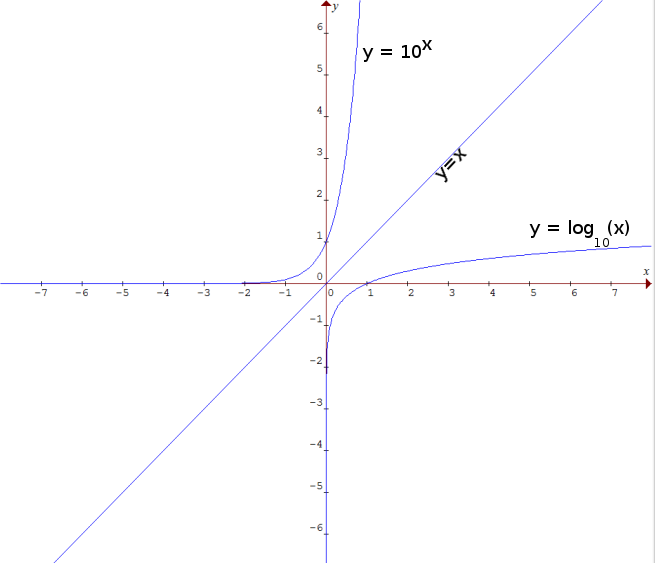
\includegraphics[width=0.5\linewidth]{1_elem_rekenvaardigheden_A/inputs/logFunc1}
	\caption{Grafische voorstelling van $y=\log_{a}(x)$.}
	\label{fig:logfunc1}
\end{figure}


\subsubsection{Grafische voorstelling van de Neperiaanse logaritme}

$y=\ln x$ is de inverse functie van $y=e^x$. Grafisch uit zich dit door spiegeling van de grafieken tegenover de eerste bissectrice $y=x$, zie ook Figuur \ref{fig:logfunc2}.

\begin{figure}
	\centering
	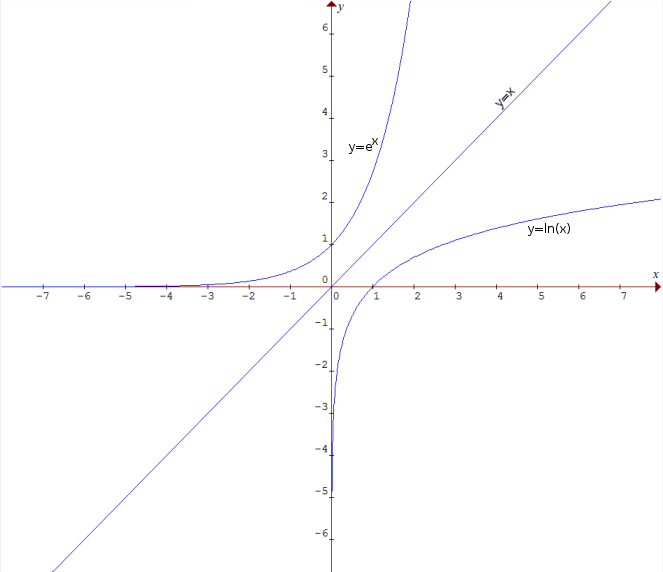
\includegraphics[width=0.5\linewidth]{1_elem_rekenvaardigheden_A/inputs/logFunc2}
	\caption{Grafische voorstelling van de Neperiaanse logaritme.}
	\label{fig:logfunc2}
\end{figure}


\subsubsection{Rekenregels:}

\fbox{\begin{minipage}{\linewidth}
	Rekenregels: \\
	
	\begin{eqnarray*}
	\log_{a}(x \cdot y) &=& \log_{a}(x) + \log_{a}(y) \\
	\log_{a}(\frac{x}{y}) &=& \log_{a}(x) - \log_{a}(y) \\
	\log_{a}(x^n) &=& n \cdot \log_{a}(x) \\
	\log_{a}(\sqrt[n]{x}) &=& \frac{1}{n}\log_{a}(x) \\
	\log_{a}(b) &=& \frac{1}{\log_{b}(a)} 
	\end{eqnarray*}
	\end{minipage}
}



\subsection{Algebra: het rekenen met letters}


\subsubsection{Gebruik van letters in de wiskunde}

De algebra is de kunst van het rekenen met letters. Die letters stellen
meestal getallen voor, en met getallen weet je hoe je kan rekenen:
optellen, aftrekken, vermenigvuldigen en delen. Bij algebra voeren
we dat soort operaties ook uit, alleen gebruiken we daarbij niet alleen
getallen, maar ook \emph{variabelen}. Dat zijn als het ware 'dingen'
waarvan we de waarde (nog) niet kennen of waarbij zo'n 'ding' meerdere
waarden kan aannemen. Voor de variabelen gebruiken we letters.

\noindent In de algebra worden vervolgens allerlei verbanden en structuren
onderzocht. Welke regels en eigenschappen gelden er, wat mag wel en
wat mag niet? Verzamelingen spelen hierbij een grote rol, maar ook
afbeeldingen. Door gebruik te maken van variabelen, vergelijkingen,
en dergelijke meer is het mogelijk 'algemene' uitspraken te doen over
verzamelingen en operaties. Bekende eigenschappen van rekenen met
getallen zijn de commutatieve eigenschap en de distributieve eigenschap.

\medskip{}

Voorbeeld: In het algemeen geldt voor het optellen en vermenigvuldigen
van $a$ en $b$ (natuurlijke getallen) dat:

\begin{equation*}
a + b = b + a \text{ en } a \times{} b = b \times{} a
\end{equation*}

Dat lijkt vanzelfsprekend, maar dat is het niet. Bij de operatie delen
geldt het bijvoorbeeld niet! ($12:4$ is niet hetzelfde als $4:12$)

\medskip{}

Een andere bekende eigenschap is de distributiviteit:

\begin{equation*}
a \texttimes{} (b + c) = a \texttimes{} b + a \texttimes{} c
\end{equation*}

Dat gebruiken we heel vaak, maar mag dat zomaar, wanneer wel, wanneer
niet?

Geldt dit bijvoorbeeld?

\begin{equation*}
a + (b \times{} c) = (a + b) \times{} (a + c) ???
\end{equation*}

\medskip{}


\noindent Met variabelen kunnen we ook \emph{formules} opstellen.
Stel dat we de straal van een cirkel voorstellen door de letter $r$.
Dan is de $\mathrm{omtrek}=2\pi r$ en de $\mathrm{oppervlakte}=\pi r^{2}$.
Nu kunnen we voor eender welke cirkel zijn omtrek en oppervlakte berekenen
door de waarde van $r$ te vervangen (we zeggen te \emph{substitueren})
door een getal.

\medskip{}


\noindent Een \emph{uitdrukking} is een geheel van termen bestaande
uit getallen, variabelen, bewerkingstekens (zoals $+$, $-$, $x$, $:$) en andere
wiskundige tekens (zoals haakjes): $2\pi r$, $3-8$, $2x+5$, ...

\noindent Vervolgens kunnen we twee uitdrukkingen aan elkaar gelijk
stellen. We spreken dan van een \emph{vergelijking}. Vergelijkingen
kunnen vaak worden afgeleid uit een stukje tekst (de klassieke vraagstukjes).
Als een vergelijking een variabele bevat, dan kunnen we trachten de
waarde (of alle waarden) van de variabele te vinden waardoor er een
ware bewering ontstaat als we de variabele vervangen door de gevonden
waarde(n). Dit wordt \emph{oplossen van de vergelijking} genoemd.
De waarde van de variabele heet in dit geval \emph{de wortel} of \emph{de
oplossing} van de vergelijking.

\noindent Een formule kan (en mag) meerdere variabelen en onbekenden
bevatten. \medskip{}


\uline{Voorbeeld 1}:

De oppervlakte van een rechthoek is $b.h$ waarbij $b$ de basis is,
en $h$ de hoogte.

Als je nu gegeven krijgt dat $b$ gelijk is aan 4 en $h$ gelijk is
aan 2 (we gebruiken even geen eenheden ter vereenvoudiging), dan kan
je de oppervlakte berekenen door de letters te substitueren, door
ze te vervangen door de echte waarden of echte getallen:

\begin{equation*}
\mathrm{oppervlakte}=b\cdot h=(4)\cdot(2)=8
\end{equation*}

Hoewel het hier niet echt nodig was, hebben we toch de gesubstitueerde
getallen tussen haken gezet. Je doet dit om aan te duiden dat je de
letter in zijn geheel vervangt door het getal. Bij moeilijke formules
maakt dit wel degelijk veel uit! Stel, je wil de oppervlakte van een
andere rechthoek berekenen, en je hebt gegeven dat de hoogte 2 meer
moet zijn dan de basis, of met andere woorden, $h=b+2$. Over de basis
weet je nog niets. Je kan dus enkel $h$ vervangen:

\begin{equation*}
\mathrm{oppervlakte}=b\cdot h=b\cdot(b+2)
\end{equation*}

Je ziet dus dat de letter $h$ volledig vervangen is door $b+2$,
gesymboliseerd door de haakjes.

\medskip{}


\uline{Voorbeeld 2}:

Ik heb een pot verf waarmee een oppervlakte van $5m^2$
kan geschilderd worden. Hoeveel ronde tafeltjes kan ik hiermee een
likje verf geven? De diameter van de tafeltjes is $1~m$.

Oplossing: 

We zoeken het aantal tafeltjes die volledig geschilderd kunnen worden.
Stel deze onbekende variabele voor door bijvoorbeeld $x$ (gevraagd).

We hebben voldoende verf om $~5~m^2$
te schilderen (gegeven).

De diameter $d$ van een tafeltje is 1 meter: $d=1~m$ (gegeven).

De straal $r$ van een cirkel is de helft van de diameter: $2r=d$

zodat de oppervlakte $s$ van 1 tafeltje gelijk is aan: $s=\pi r^{2}=\pi\left(\frac{d}{2}\right)^{2}=\frac{\pi d^{2}}{4}=\frac{\pi(1)^{2}}{4}=0,79~m^2$

We stellen de vergelijking op: $5=x.s$ 

en lossen deze tenslotte op naar de onbekende variabele: $x=\frac{5}{s}=\frac{5}{0,79}=6,37$

Besluit: we kunnen 6 tafeltjes schilderen (en dan blijft er nog een
klein beetje verf over).


\subsubsection{Manier van rekenen}

\begin{itemize}
	\item{Notaties}
	\begin{itemize}
		\item In het rekenen met letters wordt het puntje van de vermenigvuldiging
		vaak niet geschreven. In plaats van $a\cdot b\cdot c$ schrijf je
		$abc$. Of, in plaats van $2\cdot b$ schrijf je $2b$. Het puntje
		schrijven is niet fout, maar hoeft niet.
		\item Letters schrijf je achteraan in een uitdrukking, dus $b\cdot2\cdot c$
		schrijf je best als $2bc$. (Dit mag, want in een product mag je factoren
		van plaats verwisselen.)
		\item Vaak worden de letters die voorkomen ook in alfabetische volgorde
		geschreven. Bijvoorbeeld $yxz$ schrijf je beter als $xyz$. 
	\end{itemize}
	\noindent Deze notaties maken het meestal gemakkelijker om verder
	te rekenen, en als je je aan deze manier van schrijven houdt, ziet
	alles er meer netjes uit. Het is niet absoluut verplicht om te doen,
	maar wel aan te raden.
	
	
	\item{Eentermen en veeltermen}
	
	Een eenterm is een uitdrukking die uit 1 term bestaat, een veelterm
	bestaat uit meerdere termen, logisch toch? I.p.v. een veelterm spreken
	we ook over een polynoom.
	
	\textbullet{} $a$ en $4abcx$ zijn eentermen
	
	\textbullet{} $x^{2}+3x+1$ en $b-x$ zijn veeltermen
	
	
	\item{Som en verschil}
	
	Je kan de som of het verschil van eentermen maken, maar enkel als
	de letters of lettercombinatie in de eenterm gelijk is. Lijkt een
	cryptische regel, maar dat is het niet. 
	
	\noindent Bijvoorbeeld:
	
	\textbullet{} $a+3a=4a$ Dit gaat perfect, want de letters zijn gelijk.
	
	\textbullet{} $a+2b=?$ Dit gaat niet, $a$ en $b$ zijn verschillende
	letters. 
	
	\textbullet{} $2ab+bc=?$ Dit gaat niet want $ab$ en $bc$ zijn verschillende
	lettercombinaties. 
	
	\textbullet{} $3ab-ab=2ab$ Dit gaat perfect, want de lettercombinaties
	zijn gelijk.
	
	\textbullet{} $ab+ba=ab+ab=2ab$ Ook dit gaat, al is het met een omweg.
	Door te sorteren zie je dat de lettercombinaties gelijk zijn.
	\begin{itemize}
		\item $a+a^{2}=?$ Dit gaat niet, want de lettercombinaties zijn niet gelijk,
		eentje is een $a$ en de andere is $a^{2}$.
	\end{itemize}
	Let dus goed op bij het optellen van letters of combinaties, en sorteer
	de letters om gelijkaardige combinaties te zien. 
	
	\noindent Het optellen van veeltermen is een uitbreiding van deze
	regel. Gelijksoortige eentermen (dus met dezelfde lettercombinaties)
	tel je op: 
	\begin{itemize}
		\item \noindent $(3x+y)+(4x+z)=7x+y+z$ Enkel de eentermen van de $x$ kan
		je optellen, de rest moet je laten staan. 
		\item \noindent $(3x+y)-(a+b)=3x+y-a-b$ Jammer, hier kan je niets optellen.
	\end{itemize}
	
	\item{Producten}
	
	Producten van verschillende letters vorm je door de letters achter
	elkaar te schrijven. De bijhorende getallen vermenigvuldig je ook,
	en plaats je voorop. 
	
	\noindent Voor eentermen is dit:
	
	\textbullet{} $a\cdot b\cdot x=abx$ 
	
	\textbullet{} $x\cdot2a\cdot2b=4abx$ \medskip{}
	
	
	\noindent Als de letters gelijk zijn, kan je machten vormen. Je gebruikt
	hier eigenlijk de rekenregel: ``machten met hetzelfde grondtal vermenigvuldigen
	is de exponenten optellen''.
	\begin{itemize}
		\item \noindent $a\cdot a=a^{2}$
		\item \noindent $x^{2}\cdot x^{3}=x^{2+3}=x^{5}$
		\item \noindent $ab\cdot ab=(ab)^{2}=a^{2}\cdot b^{2}=a^{2}b^{2}$
	\end{itemize}
	\noindent Veeltermen vermenigvuldigen is lastiger, maar maakt gebruik
	van rekenregels die je al kent. De belangrijkste is de distributiviteit.
	Op die manier herleid je het probleem naar het product van eentermen:
	\begin{equation*}
	x\cdot(a+b)=x\cdot a+x\cdot b=ax+bx
	\end{equation*}
%	\begin{itemize}
%		\item \noindent $x\cdot(a+b)=x\cdot a+x\cdot b=ax+bx$
%	\end{itemize}
	\noindent Iets complexer: nog enkele voorbeelden:
	
	\begin{math}
	\begin{array}{ccc|r}
	(a+2x)\cdot(3x) & = & a\cdot(3x)+(2x)\cdot(3x) & \text{ distributiviteit}\\
	& = & 3ax+6x^{2} & \text{uitrekenen en ordenen}\\
	& & & \\
	(a+b)\cdot(a+b) & = & a\cdot a+b\cdot a+a\cdot b+b\cdot b &  \text{distributiviteit}\\
	& = & a^{2}+ba+ab+b^{2} &  \text{uitrekenen}\\
	& = & a^{2}+2ab+b^{2} &  \text{ordenen en optellen}\\
	& &  & \\
	(a+b)\cdot(x+y) & = & a\cdot x+a\cdot y+b\cdot x+b\cdot y=ax+ay+bx+by\\
	\end{array}
	\end{math}
	

	\noindent In module {*}{*}{*}{*} gaan we kijken naar de omgekeerde
	bewerkingen: ontbinden in factoren (afzonderen van eentermen en veeltermen),
	en merkwaardige producten.
	
	
	\item{Quoti\"enten}
	
	Quoti\"enten, en dus daarmee samenhorend breuken, bereken je vaak door
	vereenvoudigingen. Je doet een vereenvoudiging net op dezelfde manier
	als bij het vereenvoudigen van een breuk met gewone getallen:
	
	\begin{eqnarray*}
		\frac{6}{15} & = & \frac{2.3}{3.5} = \frac{2}{5}\\
		\frac{ab}{bc} & = & \frac{a}{c} \\
	\end{eqnarray*}
	

	\noindent Als er in de teller een letter staat die ook in de noemer
	staat, kan je de breuk vereenvoudigen. Maar de volgende breuk kan
	je NIET vereenvoudigen:
	
	\begin{equation*}
		{\displaystyle \frac{ab}{bc+1}}
	\end{equation*}
	
	\noindent In de noemer staat immers niet bij elke term een $b$, dus
	is vereenvoudiging hier niet mogelijk. Wat je echter wel kan (en mag
	doen) is zowel in teller als noemer de letter $b$ buiten de haakjes
	brengen; daarna kan je $b$ schrappen, maar of je daarmee de breuk
	vereenvoudigd hebt, laten we in het midden. De variabele $b$ mag
	nu immers niet meer nul worden.
	
	\begin{equation*}
	{\displaystyle \frac{ab}{bc+1}={\displaystyle \frac{ab}{b(c+\frac{1}{b})}=\frac{a}{c+\frac{1}{b}}}}
	\end{equation*}
	
	\medskip{}
	
	
	\noindent Het gebruik van rekenregels heb je echt nodig bij machten:
	
	\noindent ${\displaystyle \frac{a^{3}}{a^{2}}=a^{3-2}=a^{1}=a}$
	
	\noindent \medskip{}
	
	
	\noindent Nog een voorbeeld:
	
	\begin{math}
	\begin{array}{ccc|r}
	{\displaystyle \frac{p\sqrt{p}}{p^{2}}} & = & {\displaystyle \frac{p.p^{\frac{1}{2}}}{p^{2}}} &   \text{vierkantswortel omzetten in macht}\\
	& = & {\displaystyle \frac{p^{1+\frac{1}{2}}}{p^{2}}} &  \text{product van machten met gelijk grondtal is exponenten optellen}\\
	& = & {\displaystyle \frac{p^{\frac{3}{2}}}{p^{2}}} &  \\
	& = & {\displaystyle p^{\frac{3}{2}-2}} &  \text{quoti\"ent van machten met gelijk grondtal is exponenten aftrekken}\\
	& = & {\displaystyle p^{-\frac{1}{2}}} &  \text{Verder dan dit kan je de opgave niet vereenvoudigen.}\\
	\end{array}
	\end{math}
	
	\noindent Als je iets meer ervaring hebt: ${\displaystyle \frac{p\sqrt{p}}{p^{2}}=p^{1+\frac{1}{2}-2}={\displaystyle p^{-\frac{1}{2}}}}$.
	
\end{itemize}


\subsubsection{Voorbeelden}

\noindent Rekenen met letters kan dan wel op dezelfde manier gaan
zoals rekenen met getallen, toch is er vaak een moeilijkheid bij vereenvoudigingen
en dergelijke. Vandaar dat we enkele voorbeelden bekijken.

\begin{itemize}
	\item{Breuken optellen en aftrekken}
	
	\noindent Net zoals bij de gewone breuken, is de sleutel hier het
	op dezelfde noemer brengen van de breuken:
	
	\begin{equation*}
	{\displaystyle \frac{4}{a}+\frac{7}{a}=\frac{11}{a}}
	\end{equation*}
	
	\noindent Volgend voorbeeld is iets lastiger:
	
	\begin{equation*}
		{\displaystyle \frac{a}{b}+\frac{c}{d}}
	\end{equation*}
	
	\noindent Je zoekt hier een gelijke noemer. Omdat de noemers niets
	met mekaar te maken hebben, neem je gewoon het product van de noemers
	als gemeenschappelijke noemer, namelijk $b\cdot d$. Dat zou je ook
	doen als je de som $\frac{1}{7}+\frac{2}{3}$ zou moeten oplossen,
	dan zou je ook als gemeenschappelijke noemer $3\cdot7=21$ kiezen.
	
	\begin{equation*}
		{\displaystyle \frac{a}{b}+\frac{c}{d}=\frac{ad}{bd}+\frac{cb}{bd}=\frac{ad+bc}{bd}}
	\end{equation*}
		
	\noindent Een iets moeilijker voorbeeld:
	
	\begin{eqnarray*}
		{\displaystyle \frac{y}{x}+\frac{y}{x+1}} & = & {\displaystyle \frac{y.(x+1)}{x.(x+1)}+\frac{y.x}{(x+1).x}} \\
		& = & {\displaystyle \frac{xy+y}{x.(x+1)}+\frac{xy}{(x+1).x}} \\
		& = & {\displaystyle \frac{xy+y+xy}{x.(x+1)}} \\
		& = & {\displaystyle \frac{2xy+y}{x(x+1)}} \\
		& = & {\displaystyle \frac{2xy+y}{x^{2}+x}} 
	\end{eqnarray*}
	We werken hier ook de noemer uit.
	
	
	\noindent \medskip{}
	Nog een laatste voorbeeld:
	
	\begin{equation*}
	{\displaystyle \frac{x+3+a}{a+1}-\frac{2x+5-b}{2a+2}}
	\end{equation*}
	
	\noindent In dit voorbeeld is de gemeenschappelijke noemer gelijk
	aan $2a+2$, en niet meteen het product van de twee noemers! Immers,
	de twee noemers hebben een gemeenschappelijk factor, namelijk $a+1$.
	Daar moet je gebruik van maken. Concreet betekent dit dat we de eerste
	breuk in teller en noemer moeten vermenigvuldigen met 2, en de tweede
	noemer kunnen we gewoon laten staan:
	
	\begin{math}
	\begin{array}{ccl|r}
	{\displaystyle \frac{x+3+a}{a+1}-\frac{2x+5-b}{2a+2}} & = & {\displaystyle \frac{(x+3+a).2}{(a+1).2}-\frac{2x+5-b}{2a+2}}  & \text{op gelijke noemer zetten}\\
	& = & {\displaystyle \frac{2x+6+2a}{2a+2}-\frac{2x+5-b}{2a+2}} &\text{uitrekenen}\\
	& = & {\displaystyle \frac{2x+6+2a-(2x+5-b)}{2a+2}} & \text{ verschil van tellers, vergeet geen haken!}\\
	& = & {\displaystyle \frac{2x+6+2a-2x-5+b}{2a+2}} & \text{minteken verdelen over termen}\\
	& = & {\displaystyle \frac{1+2a+b}{2a+2}} & \text{gelijkaardige termen optellen}\\
	\end{array}
	\end{math}
	
	
	\item{Breuken vermenigvuldigen en delen}
	
	Breuken vermenigvuldigen en delen is eenvoudiger dan optellen en aftrekken;
	opnieuw gebruik je dezelfde rekenregels als voordien. 
	
	\noindent Vermenigvuldigen van breuken is tellers met tellers en noemers
	met noemers vermenigvuldigen:
	
	\begin{equation*}
		{\displaystyle \frac{a}{b}\cdot\frac{2}{x}=\frac{a.2}{b.x}=\frac{2a}{bx}} 
	\end{equation*}
	
	\noindent Een getal delen door een breuk is vermenigvuldigen met het
	omgekeerde van die breuk:
	
	\begin{equation*}
		{\displaystyle \frac{a}{b}:\frac{2}{x}=\frac{a}{b}.\frac{x}{2}=\frac{a.x}{b.2}=\frac{ax}{2b}}
	\end{equation*}	
	
	\noindent Ietsje moeilijker:
	
	\begin{math}
		\centering
	\begin{array}{ccc|r}
	{\displaystyle \frac{a+b}{c+d}.\frac{x+1}{y+1}} & = & {\displaystyle \frac{(a+b)}{(c+d)}.\frac{(x+1)}{(y+1)}} & \text{breuken vermenigvuldigen}\\
	& = & {\displaystyle \frac{ax+a+bx+b}{cy+c+dy+d}} & \text{uitrekenen}\\
	\end{array}
	\end{math}
	
%	\begin{tabular}{|c|c|c|c|r|}
%		\hline 
%		{\displaystyle \frac{a+b}{c+d}.\frac{x+1}{y+1}}$ & $=$ & ${\displaystyle \frac{(a+b)}{(c+d)}.\frac{(x+1)}{(y+1)}}$ &  & breuken vermenigvuldigen\\
%		\hline 
%		& $=$ & ${\displaystyle \frac{ax+a+bx+b}{cy+c+dy+d}}$ &  & uitrekenen\\
%		\hline 
%	\end{tabular}\medskip{}
	
	
	\noindent Vergeet ook niet (indien mogelijk) om nadien te vereenvoudigen:
	
	\begin{math}
	\centering
	\begin{array}{ccc|r}
	{\displaystyle \frac{2a+4x}{4b}:\frac{b}{2y}} & = & {\displaystyle \frac{2a+4x}{4b}.\frac{2y}{b}} & \text{ vermenigvuldigen met omgekeerde}\\
	& = & {\displaystyle \frac{(2a+4x).(2y)}{(4b).(b)}} & \text{breuken vermenigvuldigen}\\
	& = & {\displaystyle \frac{4ay+8xy}{4b^{2}}} &  \text{uitrekenen}\\
	& = & {\displaystyle \frac{ay+2xy}{b^{2}}} & \text{vereenvoudigen}\\
	\end{array}
	\end{math}
	
	\item{Machten en wortels}
	
	\begin{math}
	\begin{array}{ccccc}
	(2a)^{4} & = & 2^{4}.a^{4} &=& 16a^{4} \\
	\sqrt{16a} & = & \sqrt{16}.\sqrt{a}&=&4\sqrt{a} \\
	\left(\frac{a+2}{3}\right)^{2} & = &  \frac{(a+2)^{2}}{3^{2}}&=&\frac{a^{2}+4a+4}{9} \\
	\left(\frac{b}{1-a}\right)^{-2} & = &  \left(\frac{1-a}{b}\right)^{2}&=&\frac{(1-a)^{2}}{b^{2}}=\frac{1-2a+a^{2}}{b^{2}} \\
	\end{array}
	\end{math}
	
\end{itemize}


\subsection{Evenredigheden en de regel van drie}


\subsubsection{De regel van drie}

In een aantal vraagstukken worden er twee grootheden met elkaar vergeleken.
Deze twee grootheden houden dikwijls verband met elkaar. Dit wil zeggen
als de ene grootheid groter wordt, vermeerdert ook de andere. En als
de ene grootheid kleiner wordt, vermindert de andere grootheid eveneens.
We zeggen dat de twee grootheden zich \emph{evenredig} verhouden tot
elkaar (symbooltje $\sim$).\medskip{}


\uline{Voorbeeld 1}: 

Een doos ballonnen bevat 75 ballonnen en kost \EUR{10}. Hoeveel kosten
dan 90 ballonnen?

Er is een verband, want als de ene grootheid (= het aantal ballonnen)
vermeerdert, vermeerdert hier ook de andere grootheid (= de prijs
van de ballonnen). Hoe meer ballonnen je wil, hoe meer je zal moeten
betalen. Zulke vraagstukken kan je oplossen met de zogenaamde \emph{regel
van drie}. Bij dit soort opgaven ken je altijd 3 getallen en moet
je het vierde getal berekenen, vandaar...

\medskip{}

$\begin{array}{ccc}
75 ~\text{ballonnen} & \sim & \text{\EUR{10}} \\
1 ~\text{ballon} & \sim & \frac{\text{\EUR{10}}}{75 \text{ ballonnen}} \\ 
90 ~\text{ballonnen} & \sim & \frac{\text{\EUR{10}}}{75 \text{ ballonnen}}.90 \text{ ballonnen} = \text{\EUR{12}}\\ 
\end{array}$

Antwoord : Voor 90 ballonnen betaal je dan \EUR{12}.

Infeite ga je eerst op zoek naar de ``eenheidsprijs'' voor \'e\'en ballon:
\EUR{10} voor 75 ballonnen komt overeen met $10/75=0,133\frac{\text{EUR}}{\text{ballon}}$.
We kunnen ons ook afvragen hoeveel ballonnen je kan kopen voor \'e\'en
euro: $75/10=7,5\frac{\text{ballonnen}}{\text{EUR}}$ (praktisch zou dit betekenen dat je met \'e\'en euro 7 ballonnen kan kopen; je betaalt daarvoor $7.0,133=\text{\EUR{0.93}}$
en je houdt nog 6 eurocent over). \bigskip{}


We zeggen dat een verhouding \emph{omgekeerd evenredig} is wanneer
een vermeerdering langs de ene kant, een even grote vermindering aan
de andere kant veroorzaakt. 

\medskip{}


\uline{Voorbeeld 2}: 

Stel, ik heb voldoende veevoeder om 35 varkens gedurende 22 dagen
te voeren. Hoeveel dagen kom ik toe met dezelfde hoeveelheid veevoeder
als ik plots 70 varkens zou hebben?

Er is een verband, want als de ene grootheid (= het aantal varkens)
vermeerdert, vermindert hier de andere grootheid (= het aantal dagen
voederen). Zulke vraagstukken kan je eveneens oplossen met de regel
van drie. \medskip{}


%$\begin{array}{ccc}
%\text{veevoeder voor 35 varkens} & \sim & 22 \text{dagen} \\
%1 ~\text{ballon} & \sim & \frac{\text{\EUR{10}}}{75 \text{ ballonnen}} \\ 
%90 ~\text{ballonnen} & \sim & \frac{\text{\EUR{10}}}{75 \text{ ballonnen}}.90 \text{ ballonnen} = \text{\EUR{12}}\\ 
%\end{array}$

\begin{tabular}{lclcc}
veevoeder voor 35 varkens & $\sim$ & 22 dagen &  & \\
veevoeder voor 1 varken & $\sim$ & 22 dagen.veevoeder voor 35 varkens &  & \\
veevoeder voor 70 varkens & $\sim$ & $\frac{22\:\mathrm{dagen}.\mathrm{veevoeder\:voor}\:35\:\mathrm{varkens}}{\mathrm{veevoeder\:voor}\:70\:\mathrm{varkens}}$ & = & 11 dagen\\
\end{tabular}

Antwoord : Met dezelfde hoeveelheid veevoeder kan je $70$ varkens $11$
dagen lang voederen. \bigskip{}


Dit is dus niet hetzelfde als: Stel, ik heb veevoeder om $35$ varkens
gedurende $22$ dagen te voeren. Hoeveel veevoeder heb ik nodig om $70$
varkens te voederen gedurende diezelfde $22$ dagen?

Antwoord: de exacte hoeveelheid veevoeder in kg (dat een varken per
dag nodig heeft) kennen we niet, dus kunnen we ook niet in ``zoveel
kg'' antwoorden, maar als het aantal varkens verdubbelt, dan zal
de hoeveelheid veevoeder ook moeten verdubbelen. De verhouding ``hoeveelheid
veevoeder per varken'' verandert niet; we zeggen dat de verhouding
constant blijft. In symbolen:

\begin{equation*}
\frac{\mathrm{hoeveelheid\:veevoeder\:x}}{35\:\mathrm{varkens}}=\frac{\mathrm{hoeveelheid\:veevoeder\:y}}{70\:\mathrm{varkens}}=\text{constant}
\end{equation*}

Schrijven we dit iets anders: 
\begin{equation*}
\frac{70\:\mathrm{varkens}}{35\:\mathrm{varkens}}=\frac{\mathrm{hoeveelheid\:veevoeder\:y}}{\mathrm{hoeveelheid\:veevoeder\:x}}=\text{constant}=2
\end{equation*}

Besluit: de hoeveelheid veevoeder voor $70$ varkens = $2$ . hoeveelheid
veevoeder voor $35$ varkens.\medskip{}

Dit vraagstukje laat zien wat we bedoelen met ``kruiselings vermenigvuldigen''.

\subsubsection{Kruiselings vermenigvuldigen}

Kruiselings vermenigvuldigen is de benaming voor een rekenkundige handeling om een vergelijking tussen twee verhoudingen (evenredigheid) te vereenvoudigen. Daarbij wordt de noemer van het linkerlid vermenigvuldigd met de teller van het rechterlid, en de teller van het linkerlid vermenigvuldigd met de noemer van het rechterlid. Beide vermenigvuldigingen stelt men dan aan elkaar gelijk. De vergelijking  wordt door kruislings vermenigvuldigen vereenvoudigd tot $20y=40$, waaruit weer volgt dat $y=2$.

In formulevorm:

\begin{equation*}
\frac{a}{b} = \frac{c}{d} \Rightarrow ad = bc
\end{equation*}

Indien $bc \neq 0$ geldt ook het omgekeerde:

\begin{equation}
ad=bc \Rightarrow \frac{a}{b}=\frac{c}{d}
\end{equation}

De achtergrond van dit ''trucje'' is dat beide zijden van de vergelijking met hetzelfde re\"ele getal vermenigvuldigd kunnen worden, zonder dat de vergelijking verandert. In bovenstaande formulering kunnen beide zijden met het getal ''$bd$'' vermenigvuldigd worden, waarna volgt $ad=bc$.

\subsection{Rekenen met percentages en promillages}

$x$ percent of $x\%$ van een getal $y$ betekent: ${\displaystyle \left(\frac{x}{100}\right).y}$

\noindent $x$ promille of $x$ \textpertenthousand van een getal $y$ betekent:
${\displaystyle \left(\frac{x}{1000}\right).y}$

\noindent Een percentage of promillage heeft dus altijd betrekking
op een getal. $10\%$ op zich heeft m.a.w. eigenlijk geen betekenis.

\medskip{}


\uline{Voorbeelden}:

Hoeveel is $25\%$ van 50? Dit is: ${\displaystyle \left(\frac{25}{100}\right).50=0,25.50=12,5}$

Stel, de basisprijs van een product is $\EUR{82}$. Er komt
echter nog $21\%$ BTW bij. Aan welke prijs wordt dit product te koop
aangeboden?

Antwoord: ${\displaystyle 82+21\%\:\mathrm{van\:}82=82+17,22=\EUR{99,22}}$.

Dit soort berekeningen kan je vlotter maken via: $1,21*82=\EUR{99,22}$.
Dus als een hoeveelheid met $21\%$ toeneemt hoort daar de factor
$1,21$ bij.

Hoeveel moeten we betalen als we $30\%$ korting krijgen op een product
dat $200\EUR$ kost? We moeten dan van de prijs $30\%$
aftrekken: ${\displaystyle 200-30\%\:\mathrm{van\:}200=200-60=\EUR{140}}$.
Ook dit gaat eenvoudiger via $0,70*200=\EUR{140}$. Met een afname
van $30\%$ komt de factor $0,70$ overeen.

\medskip{}


We hebben geluk: bovenop de $30\%$ korting krijgen we nog een extra
$5\%$ studentenkorting. Nu betalen we $0,70*0,95*200=\EUR{133}$.

Procenten van procenten tel je dus niet op, maar je vermenigvuldigt
ze met elkaar. De klant heeft dus geen $35\%$ korting gekregen, maar
slechts $1-0,7*0,95=33,5\%$.

\medskip{}


\noindent Ook een gecombineerde toename en afname worden via een vermenigvuldiging
samengevoegd.

\noindent Met hoeveel procent neemt het aantal toe als het eerst $20\%$
vermeerdert en daarna met $45\%$ vermindert?

\noindent Antwoord: bij een toename van $20\%$ hoort de factor $1,2$
en bij een afname van $45\%$ hoort de factor $0,55$. Aangezien $1,2*0,55=0,66$
zal het aantal afnemen met $34\%$ .

\medskip{}


\noindent Tijdens een garageverkoop doet een verkoper ons een aantrekkelijk
voorstel. I.p.v. 15\% korting op alle spullen, krijgen wij een korting
van $\EUR{125}$ op het nog nieuwe televisietoestel dat $\EUR{1000}$
kost. We happen niet meteen toe, maar rekenen uit met hoeveel procent
125 van 1000 overeenkomt:

als $x\%\:\mathrm{van}\:y=z$

maw ${\displaystyle \left(\frac{x}{100}\right).y=z}$

dan is ${\displaystyle \frac{x}{100}}$ (of $x\%$) ${\displaystyle =\frac{z}{y}}$

In ons geval is: ${\displaystyle x=\frac{125}{1000}=0,125\:\mathrm{of}\:12,5\%}$.

We kiezen dus beter voor de $15\%$ korting!
